\input{macros}

\documentclass[a4paper,12pt,parskip=full]{scrreprt}

%\compileForSmartphone

\usepackage{acronym}
\usepackage{amsmath}
\usepackage{amssymb}
\usepackage{caption}
\usepackage{calc}
\usepackage[T1]{fontenc}
\usepackage{graphicx}
\usepackage{ifthen}
\usepackage[utf8]{inputenc}
%\usepackage[ngerman]{babel}
\usepackage{marvosym}
\usepackage{mathtools}
\usepackage{microtype}
\usepackage[colorlinks=false]{hyperref}
\usepackage{setspace}
\usepackage{subcaption}
\usepackage{tabu}
\usepackage{textcomp}
\usepackage[usenames,dvipsnames,svgnames,table]{xcolor}
\usepackage{tikz}

%\usepackage{csquotes}
%\usepackage[backend=biber,style=numeric-comp,sorting=none,maxnames=8,minnames=8,abbreviate=false]{biblatex} %sorting=nyt
%\addbibresource{literatur.bib}
%\DefineBibliographyStrings{ngerman}{
%	andothers ={{\textit{et\,al\adddot}}},
%}

\usetikzlibrary{arrows,decorations.pathreplacing}


\title{Slackforce: Documentation on the Theoretical Background}
%\subtitle{\thesisTitle}
\author{Tilman Sinning}


%\includeonly{abkuerzungsverzeichnis, einleitung,theorie,prozessierung,messverfahren,auswertung,ausblick,anhang}



\begin{document}

	\maketitle
	
	\tableofcontents

	% !TeX encoding = UTF-8
% !TeX spellcheck = en_US
% !TeX root = slackforceDocumentation.tex

\chapter{Introduction}

For slackliners it is often important to know the physical forces involved in slacklining, for example to estimate the suitability of potential slackline anchors. For static conditions, some well known calculations exist, to get the force on a slackline anchor from the sag of the slackline and the weight of the slackliner. However, it is often not easy to estimate the sag of a slackline precisely. Therefore it would be nice to have other measurement methods as well. Even more complicated is the estimation of the peak force in a slackline during dynamic movements like jumping.

The idea of the app ``Slackforce'' is to provide an easy to use solution for measuring and calculating forces in a slackline. This document describes the physical background and derivation of formulas and calculations used within this app. The app contains the following three main functionalities:

\begin{description}
	\item[Measure Force:] Measure the pretension of a slackline from the sound you hear when slapping the line with your finger.
	\item[Static Calculations:] Calculate the forces on a slackline at static conditions resulting from the geometric setup of the line.
	\item[Dynamic Simulation:] Simulate the movement and forces of a slackline during dynamic conditions like bouncing or jumping.
\end{description}

This document is divided into three chapters corresponding to the app functionalities. Note that the presented calculations are experimental and might contain errors. Use the formulas careful and do not fully trust the calculated values. The creator of this document is not responsible for any harm resulting from the use of the presented calculations and formulas.
	% !TeX encoding = UTF-8
% !TeX spellcheck = en_US
% !TeX root = slackforceDocumentation.tex

\chapter{Measure Force}

When slapping a tensioned slackline with your finger, you will hear a corresponding acoustical sound. The sound travels along the slackline as a mechanical wave and gets reflected at the end of the slackline. The propagation speed directly depends on the tension and the weight of the slackline. The idea is to calculate the pretension of the slackline from the time that sound needs to travel along the slackline back and forth. 

\section{Physical Background}

The propagation speed of a wave on a tensioned rope or slackline can be described with the following formula

\begin{equation}
v = \sqrt{\frac{F}{\mu_0}}
\label{eqn:speed1}
\end{equation}

where $v$ is the propagation speed, $F$ the force and $\mu_0$ the weight per unit length of the line. In between two sounds, the mechanical wave travels from one slackline anchor to the other and back, so it covers a distance two times the length $l$ of the line. If you measure the time of oscillation $t_{osc}$ the propagation speed can be calculated as:

\begin{equation}
	v = \frac{2\cdot l}{t_{osc}}
	\label{eqn:speed2}
\end{equation}

If you combine equation \ref{eqn:speed1} and \ref{eqn:speed2} and solve for the force you will get the following equation:

\begin{equation}
	F_0 = \frac{4\cdot l^2\cdot \mu_0}{t_{osc}^2}
	\label{eqn:measureForce}
\end{equation}

$F_0$ is the pretension of the line. As you can see, the weight and the length of the line have to be known. In the app the time of oscillation can be measured automatically with the microphone and some simple audio processing or manually by typing sound pattern on a button.

\section{The Influence of the Stretch Characteristic}

During the tensioning of the line, the line also stretches. As the total weight of the line does not change, this leads to a decrease of weight per unit length. Therefore equation \ref{eqn:measureForce} contains a systematic error on stretchy webbings. To take this into account a linear stretch behavior corresponding to the following formula is assumed.

\begin{equation}
	\frac{\Delta l}{l} = \alpha \cdot F
\end{equation}

where $\alpha$ is the stretch coefficient and $F$ is the force on the line. The corrected weight per unit length is calculated to

\begin{equation}
	\mu = \mu_0 \cdot \frac{1}{1+\alpha\cdot F}
\end{equation}

If you replace $\mu_0$ in formula \ref{eqn:measureForce} with the corrected value $\mu$ and solve the equation for F you get the following formula:

\begin{equation}
	F = \sqrt{\frac{1}{4 \alpha^2} + \frac{\mu_0\cdot 4l^2}{\alpha \cdot t_{osc}^2}} - \frac{1}{2\alpha}
	\label{eqn:measureForceWithStretch}
\end{equation}

In the App this more exact formula is used whenever a stretch coefficient greater than zero is entered.
It can be shown that formula \ref{eqn:measureForceWithStretch} equals formula \ref{eqn:measureForce} for $\alpha\rightarrow 0$.
	% !TeX encoding = UTF-8
% !TeX spellcheck = en_US
% !TeX root = slackforceDocumentation.tex

\chapter{Calculate Force} \label{sec:calculateForce}
The forces in a slackline can be obtained by using the geometric setup of the line at a given load. If the tension of the line at a given sag is known the tension at a different sag can easily be calculated with the aid of the stretch behavior.

\section{Basics} \label{sec:basics}

\begin{figure}[htb] \centering
	\includegraphics[width=0.8\textwidth]{images/slacklineWithForces.pdf}
	\caption{Schematical slackline with horizontal and vertical components of an applied force}
	\label{fig:slacklineWithForces}
\end{figure}

Figure \ref{fig:slacklineWithForces} shows a scheme of a slackline with a given length and sag. The load that is applied in the middle of the line results in a specific sag. The force on the anchor $F_a$ is determined by the vertical Force $F_v$ and horizontal force $F_h$ as shown in Figure \ref{fig:slacklineWithForces}. The forces on the left part of the line correspond to the shown forces on the right side. The total force is the sum of the forces on the left and the right side. The horizontal components eliminate each other while the vertical ones add up. If a slackliner is standing on the line, the total vertical force corresponds to the slackliner's weight. From the geometric properties shown in figure \ref{fig:slacklineWithForces} the following equation can easily be derived:


\begin{equation}
	\frac{F_a}{0.5\cdot F_v} = \frac{l_1}{s} = \frac{\sqrt{\frac{l^2}{4} + s^2}}{s}
\end{equation}

Together with the gravity acceleration $g = 9.81\frac{m}{s^2}$ and the weight of the slackliner $m$ this leads to the following four equations:

\begin{spreadlines}{1.5\baselineskip}
\begin{align}
	F &= \frac{\sqrt{s^2 + \frac{l^2}{4}}}{2\cdot s} \cdot m\cdot g \label{eqn:calcForce} \\
	m &= \frac{2\cdot s\cdot F}{g\cdot\sqrt{s^2 + \frac{l^2}{4}}} \label{eqn:calcWeight} \\
	s &= \sqrt{ \frac{m^2\cdot l^2\cdot g^2}{4\cdot(4F^2 - m^2g^2)} } \label{eqn:calSag} \\
	l &= \sqrt{ \frac{4\cdot s\cdot (4F^2 - m^2g^2)}{m^2g^2} } \label{eqn:calcLength} 
\end{align}
\end{spreadlines}

With Equation \ref{eqn:calcForce} - \ref{eqn:calcLength} it is possible to calculate any of the parameters force, weight of slackliner, sag and length, if the other parameters are known.

\section{Calculating the Pretension}

\begin{figure}[htb] \centering
	\includegraphics[width=0.8\textwidth]{images/forceStretchDiagram.pdf}
	\caption{Force-Stretch-Diagramm of a 100\,m Type 18 Line with 4,5\,kN Pretension}
	\label{fig:forceStretchDiagramm}
\end{figure}

If you know the (walking) tension of a slackline with a person standing in the middle and the stretch behavior, it is possible to calculate the pretension. Figure \ref{fig:forceStretchDiagramm} shows the stretch behavior of a Type 18 MKII line as an example. It can be seen that the stretch is not linear. To get the pretension of the line you need to know the increase of length $\Delta l$ due to the sag of the line. This can be calculated with the following formula:

\begin{equation}
	\Delta l = 2\cdot l_1 - l= 2\cdot \sqrt{s^2+\frac{l^2}{4}} - l
	\label{eqn:deltaL}
\end{equation}

To get the pretension you have to do the following steps:

\begin{enumerate}
	\item Calculate the anchor force with a slackliner on the line
	\item Read the corresponding stretch from the force-stretch-diagram
	\item Calculate the new stretch with formula \ref{eqn:deltaL}
	\item Read the pretension from the force-stretch-diagram
\end{enumerate}

If a linear stretch behavior $\frac{\Delta l}{l} = \alpha\cdot F$ is assumed, it is possible to put that relation into an analytic formula:

\begin{equation}
	F = F_0 + \frac{2\cdot \sqrt{s^2+\frac{l^2}{4}} - l}{\alpha\cdot l}
\end{equation}

However, the app always uses the force-stretch-diagram if available, as the results are better with that method.  Unfortunately some slackline manufacturers provide very little information on the stretch behavior of their lines and only a few data points are available. The app interpolates those data points linear for the calculations.

\section{Rodeo Lines}

Rodeo Lines are slacklines with a lot of sag and no pretension. So the pretension $F_0$ is always zero and the line has an initial sag $s_0$ without any slackliner standing on the line. When a slackliner steps on the line, it might stretch further and lead to a sag greater than the initial sag. Figure \ref{fig:RodeoLineWithForces} shows the forces on an rodeo line.

\begin{figure}[htb] \centering
	\includegraphics[width=0.8\textwidth]{images/rodeoLineWithForces.pdf}
	\caption{Schematical rodeo line with horizontal and vertical components of force}
	\label{fig:RodeoLineWithForces}
\end{figure}

As it can be seen there is no change to the static forces with a slackliner on the line from figure \ref{fig:slacklineWithForces}. So all the calculations of the section ``\nameref{sec:basics}'' are still valid. If you want to do calculations based on the force-stretch-diagram you have to be aware that equation \ref{eqn:deltaL} now changes to

\begin{equation}
	\Delta l = 2\cdot (l_2 - l_1) = 2\cdot \left( \sqrt{s^2+\frac{l^2}{4}} - \sqrt{s_0^2+\frac{l^2}{4}}\right)
	\label{eqn:deltaLRodeo}
\end{equation}

In addition there is no pretension to calculate, but you can calculate the initial sag of the line using the force-stretch-diagram. Therefore you have to read the stretch $\Delta l$ from the diagram and use the following formula:

\begin{align}
	s_0 &= \sqrt{l_1^2 - \frac{l^2}{4}} = \sqrt{\left(l_2-\Delta l\right)^2 - \frac{l^2}{4}} \\
	&= \sqrt{\left( \sqrt{s^2 + \frac{l^2}{4}}  -\Delta l\right)^2 - \frac{l^2}{4}}
\end{align}

\section{Calculating Slackline Forces from the Pretension}

Unfortunately it is very difficult for linear stretch behavior and impossible for a custom stretch behavior to get an analytic expression of the walking tension, that is a function of the pretension. Therefore some kind of approximation algorithm has to be used. The App is currently using the Illinois algorithm.

\section{Slackliner who is not in the middle of the Line (not implemented)}

In the following it is assumed, that the slackliner is standing at a position $p \in [0,1]$ on the line. The forces are always calculated for the left anchor point. The forces at the right anchor point equal the forces at the left anchor point at position $1-p$. Figure \ref{fig:slacklineWithForcesUnsymmetric} shows the forces in this new setup. If the slackliner is not moving, the horizontal forces have to be the same on both sides. That leads to different vertical forces and anchor forces on both sides.

\begin{figure}[htb] \centering
	\begin{subfigure}{\textwidth} \centering
		\includegraphics[width=0.8\textwidth]{images/slacklineWithForcesUnsymmetricRightSide.pdf}
	\end{subfigure} \par\bigskip
	\begin{subfigure}{\textwidth} \centering
		\includegraphics[width=0.8\textwidth]{images/slacklineWithForcesUnsymmetricLeftSide.pdf}
	\end{subfigure}
	\caption{Force Components on Unsymmetric Conditions }
	\label{fig:slacklineWithForcesUnsymmetric}
\end{figure}

According to fig. \ref{fig:slacklineWithForcesUnsymmetric} the equation below can be derived.

\begin{equation}
	\frac{p\cdot l}{s} = \frac{F_{h,l}}{F_{v,l}} = \frac{ \sqrt{F_{a,l}^2 - F_{v,l}^2 }}{F_{v,l}}
	\label{eqn:geometricPropertiesUnsymmetric}
\end{equation}

The total vertical force is still the sum of both sides:

\begin{equation}
	F_v = F_{v,l} + F_{v,r}
	\label{eqn:verticalForce}
\end{equation}

The absolute values of both horizontal forces are the same which leads to:

\begin{equation}
	\frac{p\cdot l}{s}\cdot F_{v,l} = \frac{(1-p)\cdot l}{s}\cdot F_{v,r} 
	\label{eqn:horizontalEquality}
\end{equation}

Combining equation \ref{eqn:horizontalEquality} and \ref{eqn:verticalForce} results in:

\begin{equation}
	F_{v,l} = (1-p)\cdot F_v
	\label{eqn:leftVerticalForce}
\end{equation}

Inserting equation \ref{eqn:leftVerticalForce} in \ref{eqn:geometricPropertiesUnsymmetric} leads to the final equation

\begin{equation}
	F_{a,l} = \frac{(1-p)\cdot F_v}{s}\cdot \sqrt{(p\cdot l)^2 + s^2}
\end{equation}

For $p = 0.5$ this equation is identical to equation \ref{eqn:calcForce} from the previous section. Note that equation \ref{eqn:deltaL} now changes to

\begin{equation}
	\Delta l = \sqrt{ (p\cdot l)^2 + s^2 } + \sqrt{ (1-p)^2 l^2 + s^2 } - l
\end{equation}







	\chapter{Dynamic Force Simulation}

In the previous section the basic calculations at static conditions were described. However, often it is interesting what the maximum forces are during bouncing or jumping. On highlines the forces involved in a leashfall are also very important. As the calculation of dynamic behavior is much more complicated than on static conditions finding analytic expressions is not constructive. Therefore an simulation approach is used.


\section{Basic Idea of the simulation}
To get the forces on dynamic movements the movement of the slackliner gets separated in very small time steps and for a hole period of bouncing or jumping the current speed and position get calculated for every time step. If the time steps are small enough the acceleration of the slackliner can be assumed to be constant. That leads to the following formulas:

\begin{align}
	v(t) &= at+v_0 \\
	s(t) &= \frac{a}{2}t^2 + v_0 t + s_0
\end{align}

In addition the following relations exists:

\begin{equation}
	F = a\cdot m
\end{equation}

a is the accelaration, m the mass, v the speed and s the path. Then for every time step the following pattern is done:

\begin{enumerate}
	\item Set the sag of the slackline to the current position of  the slackliner
	\item Calculate the force affecting the slackliner $F = m\cdot g - F_{v,slackline}$
	\item Calculate the acceleration of the slackliner $a = F / m$
	\item Calculate change in speed $\Delta v = a\cdot\Delta t$
	\item Calculate change in position $\Delta s = \frac{1}{2}\cdot a\cdot\Delta t^2 + v\cdot\Delta t$
	\item Add those values to the current position and speed
\end{enumerate}

When the sign of the speed changes the slackliner is at the lowest point of the line. At this point the maximum forces on the line and the slackliner appear. Therefore the simulation can be stopped here.

\section{Improved Dynamic Model (not implemented)}

In the section above it is assumed, that the stretch behavior of the line is always the same as in the static case. In reality this is not the case and the line behaves more like a viscoelastic material. Therefore it might lead to better results assuming a model based on viscoelastic behavior for the dynamic simulations.

\begin{figure}[htb] \centering
	\includegraphics[width=0.4\textwidth]{images/dynamicStandardModel.pdf}
	\caption{Standard linear solid model}
	\label{fig:dynamicStandardModel}
\end{figure}

Figure \ref{fig:dynamicStandardModel} shows the standard linear solid model. This leads to the following differential equation:

\begin{equation}
	\sigma + \frac{\eta}{E_1+E_2}\dot\sigma = \frac{E_1E_2}{E_1+E_2}\epsilon + \frac{E_2\eta}{E_1+E_2}\dot\epsilon
	\label{eqn:standardLinearModel}
\end{equation}

$E_1$, $E_2$ are the elastic modulus of the two springs, $\sigma$ is the applied stress, $\epsilon$ is the stretch $\frac{\Delta l}{l}$ and $\eta$ is the dynamic viscosity. 

For the calculation of slacklines I like to use the stretch coefficient $\alpha = \frac{\epsilon}{F}$ instead of the elastic modulus. The relation between those parameters is:

\begin{equation}
	E = \frac{1}{\alpha\cdot A}
\end{equation}

The sum of the stretch coefficients $\alpha_1+\alpha_2$ is the static stretch coefficient $\alpha$ of the line from the previous chapters. As for slacklines the cross section $A$ is not very important it makes sense to multiply equation \ref{eqn:standardLinearModel} with $A$:

\begin{equation}
F(t) + \frac{\alpha_1\alpha_2}{\alpha}\cdot (\eta A)\cdot\dot F(t) = \frac{\epsilon(t)}{\alpha} + \frac{\alpha_1}{\alpha}\cdot (\eta A)\cdot\dot{\epsilon(t)}
\end{equation}

Rearranging this equation leads to

\begin{equation}
	\dot F(t) = \frac{-\alpha}{\alpha_1\alpha_2\cdot (\eta A)} \cdot F(t) + \frac{\epsilon (t)}{\alpha_1\alpha_2\cdot(\eta A)} + \frac{\dot{\epsilon} (t)}{\alpha_2}
\end{equation}

Now we have a linear inhomogeneous differential equation. Solving this equation for the force $F$ gives:

\begin{equation}
\begin{split}
	F(t) \insertForSmartphone{&}= e^{ \frac{-\alpha t}{\alpha_1\alpha_2\cdot (\eta A)} dt } \cdot \insertForSmartphone{\\ &}\left[ \int_0^t \left( \frac{\epsilon (t')}{\alpha_1\alpha_2\cdot (\eta A)} + \frac{\dot{\epsilon}   (t')}{\alpha_2} \right) \cdot e^{\frac{\alpha t'}{\alpha_1\alpha_2\cdot (\eta A)}} dt' + C \right]
\end{split}
\end{equation}

For the simulation the change of force $\Delta F$ between to time steps $\Delta t$ is of interest. Therefore $\Delta F = F(t+\Delta t) - F(t)$ has to be calculated:

\begin{equation}
\begin{split}
	\Delta F = F(t)\cdot \left( e^{\frac{-\alpha\cdot \Delta t}{\alpha_1\alpha_2\cdot(\eta A)}} - 1 \right) + e^{\frac{-\alpha(t+\Delta t)}{\alpha_1\alpha_2\cdot (\eta A)}} \cdot \insertForSmartphone{\\} \int_t^{t+\Delta t} \left( \frac{\epsilon (t')}{\alpha_1\alpha_2\cdot(\eta A)} + \frac{\dot{ \epsilon} (t')}{\alpha_1} \right) \cdot e^{\frac{\alpha\cdot t'}{\alpha_1\alpha_2\cdot (\eta A)}} dt'
\end{split}
\end{equation}

 If the time steps are small enough a constant stretch $\epsilon(t) = \epsilon = const$ can be assumed. The derivation of the stretch changes to $\dot{\epsilon}(t) = \frac{\Delta\epsilon}{\Delta t}$. With this simplification the remaining integral can be solved.
The result is:

\begin{equation}
	\Delta F = \left( 1 - e^{\frac{-\alpha\cdot\Delta t}{\alpha_1\alpha_2\cdot (\eta A)}} \right) \cdot \left( \frac{\epsilon}{\alpha} - F(t) + \frac{\alpha_1\cdot (\eta A)}{\alpha} \cdot \frac{\Delta\epsilon}{\Delta t} \right)
	\label{eqn:finalDynamicEquation}
\end{equation}

Equation \ref{eqn:finalDynamicEquation} can now easily be used for the simulation. The calculation of the current forces works with the following procedure.

\begin{enumerate}
	\item Initialize the force with the pretension and the stretch with the force-stretch-diagram
	\item Calculate the new position of the slackliner and sag of the line according to the previous section
	\item Calculate the new stretch and $\Delta\epsilon$ with the geometric properties of the line
	\item Calculate the new force $F(t+\Delta t) = F(t) + F(\Delta t)$ with equation \ref{eqn:finalDynamicEquation}
	\item Repeat steps 2 - 4
\end{enumerate}


To get good simulation results dynamic characterizations of some real lines are necessary. However, as a starting point I could find some dynamic parameters of climbing ropes at the following webpage (unfortunately in german): \url{http://www.sigmadewe.com/fileadmin/user_upload/pdf-Dateien/SEILPHYSIK.pdf}.
For the ropes tested there the ratio $\frac{\alpha_1}{\alpha_2}$ was always about $3$. The viscosity was varying between $\eta A = 4.8 \dots 9\,kN\cdot s$. I can imagine that slacklines might have a lower damping than climbing ropes, but that is only speculation. When I have time I will implement this model and play around with the parameters to see if I can get a good match to existing dynamic force measurements.

	

\end{document}          
